\section{Preliminaries}
This section introduces the key components of DER while describing its limitations.
We conclude this section by describing how to simulate the behavior of a cable modeled as a Deformable Linear Object (DLO).
Note more details about DER can be found at \cite{originalDER} and in the appendix to this paper.
Throughout the rest of the document, let  $|\cdot|$ represents $||\cdot||_2$ and $\times$ denote the cross product between two vectors in $\R^3$.

\subsection{DLO Model}

We model the DLO using an indexed set of $n$ vertices at each time instance. 
The ground truth locations of vertex $i$ at time $t$ is denoted by $\timevertind{x}{i}{t} \in \R^3$ and the set of all $n$ vertices is denoted by $\timeind{X}{t}$. 
Let $\textit{\textbf{M}}^\text{i}\in \mathbb{R}^{3\times3}$ denote the mass matrix of vertex $i$.
The segments of the DLO are the lines between successive vertices, $\timevertind{e}{i}{t} = \timevertind{x}{i+1}{t} - \timevertind{x}{i}{t}$, and let $\timeind{E}{t}$ correspond to the set of all vertices at time $t$.

Our objective is to model the behavior of a DLO that is being controlled by a robot and as a result we make the following assumption:
\begin{assum}
    The first and last edge of the DLO are each held by a distinct end effector of a robot 
\end{assum}
\noindent Note this assumption is commonly made during wire manipulation \cite{IRP, diminishingridgidity, directionalrigidity, inlstm, gelsim}.
Using this assumption, let the orientation and position of the two end effectors at time $t$ be denoted by $\vertindu_t \in \R^{12}$, which we refer to as the input.
Let $\textbf{U}_{1:\text{T}-1}$ denote the set of inputs applied between times $1$ and $\text{T}-1$, and let $\textbf{X}_{1:\text{T}} =\{\textbf{X}_1, \textbf{X}_2,\ldots, \textbf{X}_\text{T}\} \in \mathbb{R}^{\text{T} \times \text{n}\times 3}$ denote the associated trajectory of the DLO from times $1$ to $\text{T}$.

Let $\Delta_t$ denote the difference in time between successive elements of $\textbf{X}_{1:\text{T}}$.
Then let $\timeind{V}{t}  = (\timeind{X}{t} - \timeind{X}{t-1})/\Delta \text{t}$.
Finally note that we differentiate between ground truth elements and predicted elements by using ``hat'' (\textit{e.g.}, $\textbf{X}_{t}$ is the ground truth set of vertices at time $t$ and $\pred{X}{t}$ is the predicted set of vertices at time $t$).

\subsection{Modeling DLO with DER for Dual Manipulation}
\label{sec:DER}

\begin{figure}
    \centering
     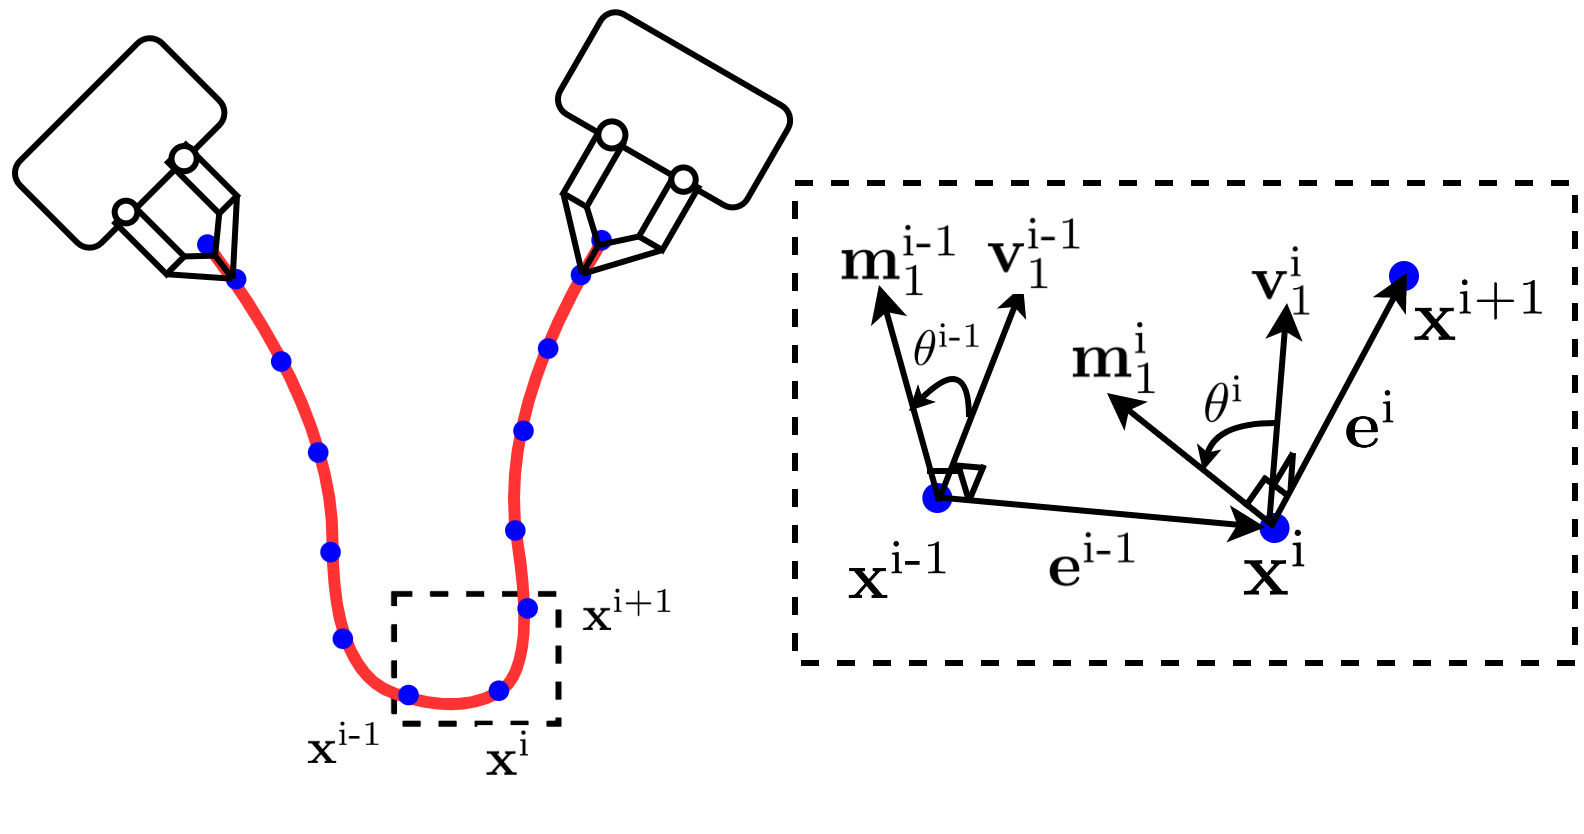
\includegraphics[width=.5\textwidth]{figures/vertices.png}
     \caption{\textbf{replace with real world image}}
    \label{fig:primal-dual}
\end{figure}

DLOs primarily exhibit three distinct modes: bending, twisting, and inextensibility \Ram{need a citation here}.
Unfortunately, accurately modeling bending and twisting is challenging without introducing numerous additional parameters (e.g., stress and strain tensors) that can make it challenging to simulate the behavior of these models in real-time \cite{twistbendchallenge, twistbendchallenge2}.
To enforce inextensibility, it is typical to apply a large stretch stiffness, but this can introduce instabilities during simulation that can make using these models for prediction difficult. 
To address these challenges, (1) DER introduces a single scalar $\theta^\text{i}_{t} \in \R$ that accurately represents bending and twisting in $\R^3$ and (2) DER enforces inextensibility using a fast, stable projection method \cite[Section 4]{fast_proj}. 
Note, as this subsection's derivation is time-invariant, the time symbol $t$ is omitted for conciseness. 


\subsubsection{Reduced Frame Modeling Using the Bishop Frame} 

Typically, DLOs are modeled using a variety of coordinate frames called \emph{configuration frames} that are located at each vertex $i$.
These are denoted by $\Gamma^{i}$ for each $i \in \{1,\ldots,n-1\}$ and
are defined by three orthonormal vectors that correspond to the coordinate axes of the frame: $\bm{t}^\text{i}, \textbf{n}^\text{i},$ and $\textbf{b}^\text{i}$.
Note $\bm{t}^\text{i}=\textbf{e}^\text{i}/|\textbf{e}^\text{i}|$, $\vertind{n}{i}$ is the normal to $\vertind{t}{i}$, and $\vertind{b}{i}=\vertind{i}{i} \times \vertind{n}{i}$. 
To model the behavior of a DLO, one typically begins by computing the energy of the cable.
One can construct an approximation of the energy of a cable by computing the energy associated with bending and twisting at each of these different coordinate frames. 

To simplify this energy computation, DER begins by defining the \emph{Bishop frame}, $\Gamma^\text{i}_\text{B}$, which corresponds to a twist-free frame (i.e., it corresponds to the frame that is not rotated with respect to the frame centered at the previous edge, so the energy associated with twisting is minimized in this frame). 
To formalize this notion, suppose the Bishop frame has coordinate axes $\textbf{t}^\text{i}, \textbf{w}_1^\text{i},$ and $\textbf{w}_2^\text{i}$ that are formally defined in the Appendix for convenience.
Let $\theta^\text{i}$ correspond to the rotation about $\vertind{t}{i}$ starting from the Bishop frame to generate a coordinate frame $\Gamma^\text{i}_\text{B}(\theta^i)$, which has coordinate axis $\textbf{t}^\text{i}, \textbf{m}_1^\text{i},$ and $\textbf{m}_2^\text{i}$ where:
\begin{align}
    \textbf{m}_1^\text{i}&=\text{cos}\theta^\text{i}\cdot \textbf{w}_1^\text{i} + \text{sin}\theta^\text{i}\cdot \textbf{w}_2^\text{i},\\
    \textbf{m}_2^\text{i}&=-\text{sin}\theta^\text{i}\cdot \textbf{w}_1^\text{i} + \text{cos}\theta^\text{i}\cdot \textbf{w}_2^\text{i}.
\end{align}
Note that  $\Gamma^\text{i}_\text{B} = \Gamma^\text{i}_\text{B}(0)$.
The Bishop frame satisfies the following lemma whose proof can be found in \Ram{please reference a specific paper's proof of this lemma}:
\begin{lem}
\label{lem:bishop_twist}
Let  $\overline{\textbf{B}}_\text{i} \in \mathbb{R}^{2 \times 2}$ denote the bending modulus of vertex $i$ which is a material property of the cable.
    Let $E_\text{twist}(\Gamma^\text{i}_\text{B}(\theta^\text{i}),\overline{\textbf{B}}_\text{i})$ denote the twisting energy of $\Gamma^\text{i}_\text{B}(\theta^i)$. 
    Then $E_\text{twist}(\Gamma^\text{i}_\text{B}(\theta^\text{i}),\overline{\textbf{B}}_\text{i})\geq E_\text{twist}(\Gamma^\text{i}_\text{B}(0),\overline{\textbf{B}}_\text{i})$ for all $\theta^i$.
\end{lem}
Similarly one can start from the Bishop frame, rotate it by $\theta^i$, and project it on the curvature binormal vector to construct the \emph{Curvature Binormal Frame}, $\Gamma^\text{i}_\text{C}(\theta^i)$. 
For conciseness, we leave the derivation of this frame to the Appendix \Ram{make sure this is done}. 
However, one can prove the following result related to the bending energy using the Curvature Binormal Frame:
\begin{lem}
\label{lem:bishop_bend}
    Let $E_\text{bend}(\Gamma^\text{i}_\text{C}(\theta^i))$ denote the bending energy of $\Gamma^\text{i}_\text{C}(\theta^i)$. 
    Then $E_\text{bend}(\Gamma^\text{i}_\text{C}(0))\geq E_\text{bend}(\Gamma^\text{i}_\text{C}(\theta^\text{i}))$ for all $\theta^i$.
\end{lem}
Lemmas \ref{lem:bishop_twist} and \ref{lem:bishop_bend} allow one to compute the energy of a DLO that arises due to bending and twisting by using Bishop and Curvature Binormal Frame rather than working directly in the configuration frame. 
\Ram{will we present the formulas for the energy somewhere and do we want to say that they are convex functions of $\theta$ or something?}
As we show in Section \ref{sec:integration}, once we compute the energy of the DLO, then we can simulate its behavior.

\subsubsection{Inextensibility Enforcement}
During simulation, the DLO's length may change, but this is not a typical property of most cables.
To ensure that the length of the DLO does not change during simulation, DER perform projection of a computed solution to ensure that the following constraint is satisfied:
\begin{equation}
    \textbf{e}_\text{i} \cdot \textbf{e}_\text{i} - \overline{\textbf{e}}_\text{i}\cdot\overline{\textbf{e}}_\text{i} = 0
\label{eq:inextensibility}
\end{equation}
where $\overline{\textbf{e}}_\text{i}$ denotes the undeformed edge. 
Unfortunately to ensure stability while performing simulation, this method requrest it to use small step sizes. 
As a result, in this paper we adopt a constraint solver based on position-based dynamics(PBD) \cite{PBD} that is described in Section\ref{sec:inextensiblity methodology}. 

\subsection{DLO Simulation Using DER}
\label{sec:integration}

To simulate the behavior of the DLO, we use DER to compute the total energy of the cable. 
Once that total energy is computed, one can apply state of the art ordinary differential equation solvers to simulate the behavior of the system.
However, to do this we need to assume that the cable reaches an equilibrium state between each simulation time step:
\begin{assum}
    The Bishop and Curvature Binormal Frame reach an equilibrium state at each time step. 
    As a result, at each time step $t$ one can compute 
    \begin{equation}
        \symbind{\theta}{i}^*_t = \underset{\theta^i_t}{\arg\min} \left(E_\text{twist}(\symbind{\Gamma}{i}_\text{B}(\theta^\text{i}_t)) + E_\text{bend}(\symbind{\Gamma}{i}_\text{C}(\theta^\text{i}_t)) \right)
        \label{eq:opt_theta}
    \end{equation}
\end{assum}

For conciseness, let $\theta_t^*$ represent all of the rotational parameters associated with the Bishop and Curvature Binormal Frames for a particular $\timeind{X}{t}$. 
Note that $\theta^*_\text{t}$ is a function of $\timeind{X}{t}$. 
As a result, the total energy of the cable at time step $t$ is:
\begin{equation}
    \text{E}(\textbf{X}_t) = \sum^{n-1}_{i=2} \left(\text{E}_{\text{twist}}(\Gamma_\text{B}^\text{i}(\symbind{\theta}{i}_t^*)) + \text{E}_{\text{bend}}(\Gamma_\text{C}^{i}(\symbind{\theta}{i}_t^*))\right) 
    \label{eq:energy}
\end{equation}
This representation enables us to perform simulation as we describe next.


Because the negative of the derivative of the total (potential) energy of the cable is equal to the force into the system, one can apply derive the following equation of motion from Newton's Second Law:
\begin{equation}
       \textit{\textbf{M}}\ddot{\textbf{X}}_{t} = -\frac{d\text{E}(\textbf{X}_t)}{d \textbf{X}_{t}}
       \label{eq:Integration}
\end{equation}
One can numerically integrate this formula to predict the velocity and position:
\begin{align}
        \hat{\textbf{V}}_{t+1} &= \hat{\textbf{V}}_\text{t}-\Delta_\text{t}m^{-1}\frac{d\text{E}(\textbf{X}_t)}{d \textbf{X}_{t}}, \\  
        \hat{\textbf{X}}_{\text{t}+1} &= \hat{\textbf{X}}_\text{t} + \Delta_\text{t}\hat{\textbf{V}}_{t+1}.
       \label{eq:Semi-Euler}
\end{align}
However, if the time step is large, it can be challenging to simulate these models accurately.
To address this challenge in \secref{sec:Differentiable DER} we develop a differentiable simulation model that enables to apply residual learning to perform predictive compensation during integration as is described in \secref{sec:integration_NN}.
% However, based on experiment and natural deficiency from large-time step discretization, we find that this method cannot capture high dynamic performance. 
% We enhance the integration approach by incorporating predictive compensation. 
% This enhancement is rooted in the concept of residual learning and is achieved through the adaptation of a graph neural network. 
% Further details will be discussed in \secref{sec:integration_NN}.
% ; however, note that our goal is to eventually perform differentiable simulation to allow for auto-tuning certain model parameters which is described in more detail in \secref{sec:Differentiable DER}.

% \subsection{Long Time Horizon Prediction for DLO}

% Following assumptions are made to setup a prediction framework.
% \begin{assum}
%     first two states $\timeind{X}{1}, \timeind{X}{2}$ are fully observable. 
% \end{assum}
% Satisfying this assumption is essential for the initialization of iterative prediction. However, when perception is heavily occluded at the initial state, meeting above assumption can be challenging. Details will be discussed in \secref{section: Estimation}
% \begin{assum}
% End edges of wire are coupled with grippers such that $\textbf{u}_\text{t}=\{\timevertind{x}{1}{t+1}, \timevertind{x}{2}{t+1}, \timevertind{x}{n-1}{t+1}, \timevertind{x}{n}{t+1}\}$. $\textbf{u}_\text{t}$ can be approximated through inverse kinematics or other perception system.
% \end{assum}
% Above assumption commonly made and well-studied in wire manipulation among literature\cite{IRP, diminishingridgidity, directionalrigidity, inlstm, gelsim}. It provides accessibility and controllability to wire edges.

%  \Ram{use an assumption environment like in the file I shared with you....} 
% \Ram{what does this mean?}. With above assumptions, denote $F$ as a general modeling function, long-time horizon inference is propagated through iterative prediction as shown in the \textbf{Algorithm} \ref{alg:long time horizon}. Note ground truth is not accessible during the iteration, and all predicted intermediate and final states of the wire will be used for evaluation. 
% \begin{algorithm}[t]
% \caption{Long Time Horizon Prediction } 
% \label{alg:long time horizon}
% \textbf{Require:} $\textbf{X}_{1:\text{T}}, \textbf{U}_{2:\text{T-1}}$ \Comment{True States and Inputs}\\
% \textbf{Initialization} at t = 2: 
% \begin{algorithmic}[1]
% \State $\textbf{V}_2 = (\textbf{X}_2 - \textbf{X}_1)/\Delta \text{t}$ \Comment{Initial Velocity Estimation } 
% \State $\pred{X}{3} = F(\textbf{u}_2, \textbf{X}_2, \textbf{V}_2)$   \Comment{First Update}
% \State $\pred{V}{3} = (\pred{X}{3} - \textbf{X}_2)/\Delta \text{t}$ \Comment{Velocity Update}
% \State {Iterative Update: $\text{T} \gg \Delta \text{t}$ \Ram{not sure why you need this condition...I think you are just running a for loop? Also isn't this just a single algorithm, why does the line number change halfway thru? Is this supposed to be two algorithms? Then call them two algorithms?}} \Yizhou{I was trying to show it is long time horizon but I can delete this line.}
% \For{$\text{t} \gets 3 \textrm{ to } \text{T}-1$} 
%      \State $\pred{X}{t+1} = F(\textbf{u}_\text{t}, \pred{X}{t}, \pred{V}{t})$
%      \State $\pred{V}{t+1} = (\pred{X}{t+1} - \pred{X}{t})/\Delta t$
% \EndFor
% \State \Return $\pred{X}{3:T}, \, |\pred{X}{3:T} - \timeind{X}{3:T}|$ \Comment{Prediction and Loss}
% \end{algorithmic}
% \end{algorithm}


% \subsection{Integration for DLO Simulation}
% \label{sec:integration}
% Notice that $\theta^*_\text{t}$ is a function of $\timeind{X}{t}$. For conciseness, based on \Eqref{eq:energy}, we note equation of motion as follows: 
% \begin{equation}
%        \textit{\textbf{M}}\ddot{\textbf{X}}_{t} = -\frac{\delta \text{E}(\Gamma^\text{M}(\timeind{X}{t}))}{\delta \textbf{X}_{t}}
%        \label{eq:Integration}
% \end{equation}
% As DER is not an analytical modeling frame. Solving  \Eqref{eq:Integration} requires numerical integration. DER\cite{originalDER} choose the method to be Semi-Euler method\cite{implicit-euler}, which has the same computational cost while having better tracking performance compared to Euler's method, as shown in the following, 
% \begin{equation}
%         \hat{\textbf{V}}_{t+1} = \textbf{V}_\text{t} -\Delta \text{t}m^{-1}\frac{\delta \text{E}(\Gamma^\text{M}(\textbf{X}_{t}))}{\delta \textbf{X}_{t}}, \, \,  \hat{\textbf{X}}_{\text{t}+1} = \textbf{X}_\text{t} + \Delta \text{t} \hat{\textbf{V}}_{t+1}
%        \label{eq:Semi-Euler}
% \end{equation}
% However, based on experiment and natural deficiency from large-time step discretization, we find that this method cannot capture high dynamic performance. We enhance the integration approach by incorporating predictive compensation. This enhancement is rooted in the concept of residual learning and is achieved through the adaptation of a graph neural network. Further details will be discussed in \secref{sec:integration_NN}.

% \subsection{Long Time Horizon Prediction for DLO}
% Following assumptions are made to setup a prediction framework.
% \begin{assum}
%     first two states $\timeind{X}{1}, \timeind{X}{2}$ are fully observable. 
% \end{assum}
% Satisfying this assumption is essential for the initialization of iterative prediction. However, when perception is heavily occluded at the initial state, meeting above assumption can be challenging. Details will be discussed in \secref{section: Estimation}
% \begin{assum}
% End edges of wire are coupled with grippers such that $\textbf{u}_\text{t}=\{\timevertind{x}{1}{t+1}, \timevertind{x}{2}{t+1}, \timevertind{x}{n-1}{t+1}, \timevertind{x}{n}{t+1}\}$. $\textbf{u}_\text{t}$ can be approximated through inverse kinematics or other perception system.
% \end{assum}
% Above assumption commonly made and well-studied in wire manipulation among literature\cite{IRP, diminishingridgidity, directionalrigidity, inlstm, gelsim}. It provides accessibility and controllability to wire edges.

%  \Ram{use an assumption environment like in the file I shared with you....} 
% \Ram{what does this mean?}. With above assumptions, denote $F$ as a general modeling function, long-time horizon inference is propagated through iterative prediction as shown in the \textbf{Algorithm} \ref{alg:long time horizon}. Note ground truth is not accessible during the iteration, and all predicted intermediate and final states of the wire will be used for evaluation. 
% \begin{algorithm}
% \caption{Long Time Horizon Prediction } 
% \label{alg:long time horizon}
% \textbf{Require:} $\textbf{X}_{1:\text{T}}, \textbf{U}_{2:\text{T-1}}$ \Comment{True States and Inputs}\\
% \textbf{Initialization} at t = 2: 
% \begin{algorithmic}[1]
% \State $\textbf{V}_2 = (\textbf{X}_2 - \textbf{X}_1)/\Delta \text{t}$ \Comment{Initial Velocity Estimation } 
% \State $\pred{X}{3} = F(\textbf{u}_2, \textbf{X}_2, \textbf{V}_2)$   \Comment{First Update}
% \State $\pred{V}{3} = (\pred{X}{3} - \textbf{X}_2)/\Delta \text{t}$ \Comment{Velocity Update}
% \State {Iterative Update: $\text{T} \gg \Delta \text{t}$ \Ram{not sure why you need this condition...I think you are just running a for loop? Also isn't this just a single algorithm, why does the line number change halfway thru? Is this supposed to be two algorithms? Then call them two algorithms?}} \Yizhou{I was trying to show it is long time horizon but I can delete this line.}
% \For{$\text{t} \gets 3 \textrm{ to } \text{T}-1$} 
%      \State $\pred{X}{t+1} = F(\textbf{u}_\text{t}, \pred{X}{t}, \pred{V}{t})$
%      \State $\pred{V}{t+1} = (\pred{X}{t+1} - \pred{X}{t})/\Delta t$
% \EndFor
% \State \Return $\pred{X}{3:T}, \, |\pred{X}{3:T} - \timeind{X}{3:T}|$ \Comment{Prediction and Loss}
% \end{algorithmic}
% \end{algorithm}


% To formulate reduced coordinate modeling, $\theta^\text{i}$ is introduced to measures the rotation about $\vertind{t}{i}$ from Bishop frame $\Gamma^\text{i}_\text{B}: {\{\textbf{t}^\text{i}, \textbf{v}_1^\text{i}, \textbf{v}_2^\text{i}\}}$ relative to material frame material frame $\Gamma^\text{i}_\text{M}:\{\boldsymbol{\textbf{t}}^\text{i}, \textbf{m}_1^\text{i}, \textbf{m}_2^\text{i}\}$ with following equation.
% \begin{equation}
%     \textbf{m}_1^\text{i}=\text{cos}\theta^\text{i}\cdot \textbf{v}_1^\text{i} + \text{sin}\theta^\text{i}\cdot \textbf{v}_2^\text{i}, \textbf{m}_2^\text{i}=-\text{sin}\theta^\text{i}\cdot \textbf{v}_1^\text{i} + \text{cos}\theta^\text{i}\cdot \textbf{v}_2^\text{i}
% \end{equation}
% Bishop frame is referred as twist-free frame according to following lemma:
% \begin{lem}
%     Let $E_\text{twist}(\Gamma^\text{i}(\theta^\text{i}))$ denote twisting energy of $\Gamma^\text{i}$. $\forall \theta^\text{i} \neq 0, E_\text{twist}(\Gamma^\text{i}_\text{M}(\theta^\text{i}))\geq E_\text{twist}(\Gamma^\text{i}_\text{M}(\theta^\text{i}=0)=\Gamma^\text{i}_\text{B})$
% \end{lem}
% Such property is critical as it allows the material frame to use Bishop frame as a reference frame (energy-minimized frame) to capture twisting efficiently. Importantly, bending energy of  material frame has following property.
% \begin{lem}
%     Let $E_\text{bend}(\symbind{\Gamma}{i}(\vertind{e}{i-1}, \vertind{e}{i}, \theta^\text{i})$ denote bending energy of $\symbind{\Gamma}{i}$. $\forall \theta^\text{i} \neq 0, E_\text{bend}(\Gamma^\text{i}_\text{M}(\vertind{e}{i-1}, \vertind{e}{i},0))\geq E_\text{bend}(\symbind{\Gamma}{i}_\text{M}(\vertind{e}{i-1}, \vertind{e}{i},\theta^\text{i}))$
% \end{lem}
% Lemma 1 and Lemma 2 allow $\theta^\text{i}$ to distribute twisting and bending energy within a bounded material frame energy. The weight of each is based on quasistatic treatment with the following assumption.
% \begin{assum}
%     The material frame always reaches an equilibrium state before simulating the next step, as $E_\text{twist}(\symbind{\Gamma}{i}_\text{M}(\theta^\text{i})) + E_\text{bend}(\symbind{\Gamma}{i}_\text{M}(\vertind{e}{i-1}, \vertind{e}{i}, \theta^\text{i}))$ is bounded, $(\symbind{\theta}{i})^*$ can always be solved with following:
%     \begin{equation}
%         (\symbind{\theta}{i})^* = \underset{\theta^i}{\arg\min}(E_\text{twist}(\symbind{\Gamma}{i}_\text{M}(\theta^\text{i})) + E_\text{bend}(\symbind{\Gamma}{i}_\text{M}(\vertind{e}{i-1}, \vertind{e}{i},\theta^\text{i})))
%         \label{eq:opt_theta}
%     \end{equation}
% \end{assum}
% Final energy is expressed as following:
% \begin{equation}
%     \text{E}(\Gamma^\text{M}(\theta^*), \textbf{E}) = \sum^{n-1}_{i=2}\text{E}_{\text{twist}}(\Gamma_\text{M}^\text{i}((\symbind{\theta}{i})^*)) + \text{E}_{\text{bend}}(\Gamma_\text{M}^{i}(\vertind{e}{i-1}, \vertind{e}{i}, (\symbind{\theta}{i})^*)) 
%     \label{eq:energy}
% \end{equation}
% Such energy formulation in reduced coordinates facilitates computation efficiency while managing to perform bending and twisting. Despite its success, notice we want to build a differentiable simulation that enables parameter auto-tuning. However, solving of Eq.\ref{eq:opt_theta} poses challenge to obtain gradients, which will be discussed in \secref{sec:Differentiable DER}.


% \subsection{Integration for DLO Simulation}
% \label{sec:integration}
% Notice that $\theta^*_\text{t}$ is a function of $\timeind{X}{t}$. For conciseness, based on \Eqref{eq:energy}, we note equation of motion as follows: 
% \begin{equation}
%        \textit{\textbf{M}}\ddot{\textbf{X}}_{t} = -\frac{\delta \text{E}(\Gamma^\text{M}(\timeind{X}{t}))}{\delta \textbf{X}_{t}}
%        \label{eq:Integration}
% \end{equation}
% As DER is not an analytical modeling frame. Solving  \Eqref{eq:Integration} requires numerical integration. DER\cite{originalDER} choose the method to be Semi-Euler method\cite{implicit-euler}, which has the same computational cost while having better tracking performance compared to Euler's method, as shown in the following, 
% \begin{equation}
%         \hat{\textbf{V}}_{t+1} = \textbf{V}_\text{t} -\Delta \text{t}m^{-1}\frac{\delta \text{E}(\Gamma^\text{M}(\textbf{X}_{t}))}{\delta \textbf{X}_{t}}, \, \,  \hat{\textbf{X}}_{\text{t}+1} = \textbf{X}_\text{t} + \Delta \text{t} \hat{\textbf{V}}_{t+1}
%        \label{eq:Semi-Euler}
% \end{equation}
% However, based on experiment and natural deficiency from large-time step discretization, we find that this method cannot capture high dynamic performance. We enhance the integration approach by incorporating predictive compensation. This enhancement is rooted in the concept of residual learning and is achieved through the adaptation of a graph neural network. Further details will be discussed in \secref{sec:integration_NN}.

% \subsection{Long Time Horizon Prediction for DLO}
% Following assumptions are made to setup a prediction framework.
% \begin{assum}
%     first two states $\timeind{X}{1}, \timeind{X}{2}$ are fully observable. 
% \end{assum}
% Satisfying this assumption is essential for the initialization of iterative prediction. However, when perception is heavily occluded at the initial state, meeting above assumption can be challenging. Details will be discussed in \secref{section: Estimation}
% \begin{assum}
% End edges of wire are coupled with grippers such that $\textbf{u}_\text{t}=\{\timevertind{x}{1}{t+1}, \timevertind{x}{2}{t+1}, \timevertind{x}{n-1}{t+1}, \timevertind{x}{n}{t+1}\}$. $\textbf{u}_\text{t}$ can be approximated through inverse kinematics or other perception system.
% \end{assum}
% Above assumption commonly made and well-studied in wire manipulation among literature\cite{IRP, diminishingridgidity, directionalrigidity, inlstm, gelsim}. It provides accessibility and controllability to wire edges.

%  \Ram{use an assumption environment like in the file I shared with you....} 
% \Ram{what does this mean?}. With above assumptions, denote $F$ as a general modeling function, long-time horizon inference is propagated through iterative prediction as shown in the \textbf{Algorithm} \ref{alg:long time horizon}. Note ground truth is not accessible during the iteration, and all predicted intermediate and final states of the wire will be used for evaluation. 
% \begin{algorithm}
% \caption{Long Time Horizon Prediction } 
% \label{alg:long time horizon}
% \textbf{Require:} $\textbf{X}_{1:\text{T}}, \textbf{U}_{2:\text{T-1}}$ \Comment{True States and Inputs}\\
% \textbf{Initialization} at t = 2: 
% \begin{algorithmic}[1]
% \State $\textbf{V}_2 = (\textbf{X}_2 - \textbf{X}_1)/\Delta \text{t}$ \Comment{Initial Velocity Estimation } 
% \State $\pred{X}{3} = F(\textbf{u}_2, \textbf{X}_2, \textbf{V}_2)$   \Comment{First Update}
% \State $\pred{V}{3} = (\pred{X}{3} - \textbf{X}_2)/\Delta \text{t}$ \Comment{Velocity Update}
% \State {Iterative Update: $\text{T} \gg \Delta \text{t}$ \Ram{not sure why you need this condition...I think you are just running a for loop? Also isn't this just a single algorithm, why does the line number change halfway thru? Is this supposed to be two algorithms? Then call them two algorithms?}} \Yizhou{I was trying to show it is long time horizon but I can delete this line.}
% \For{$\text{t} \gets 3 \textrm{ to } \text{T}-1$} 
%      \State $\pred{X}{t+1} = F(\textbf{u}_\text{t}, \pred{X}{t}, \pred{V}{t})$
%      \State $\pred{V}{t+1} = (\pred{X}{t+1} - \pred{X}{t})/\Delta t$
% \EndFor
% \State \Return $\pred{X}{3:T}, \, |\pred{X}{3:T} - \timeind{X}{3:T}|$ \Comment{Prediction and Loss}
% \end{algorithmic}
% \end{algorithm}



% The bishop frame is defined as following:
% \begin{defn}
%     \label{def: Bishop}
%      Denote $\bm{v^\text{i+1}} = R_{\text{q}^\text{i}}(\bm{v^\text{i}}), \, \text{q}^\text{i}=(\text{q}_0^\text{i}, \textbf{q}^\text{i})$ as quaternion rotation that rotates $\bm{v^\text{i}}$ around axial vector $\textbf{q}^\text{i}$ with magnitude $\text{q}_0^\text{i}$. Let $\phi^\text{i}$ denote the turning angle between $\vertind{e}{i}$ and $\vertind{e}{i+1}$. Given 
% \begin{equation}
% \textbf{t}^{\text{i}+1} =R_{\text{q}^\text{i}}(\textbf{t}^\text{i}),\, \textbf{n}_1^{\text{i}+1} \label{eq:parallel transfort1} =R_{\text{q}^\text{i}}(\textbf{n}_1^\text{i})
% \end{equation}  
% \begin{equation}
% \text{q}_0^\text{i} = \text{cos}(\phi^\text{i}/2), \, \textbf{q}^\text{i} = \text{sin}(\phi^\text{i}/2)(\textbf{t}^\text{i} \times \textbf{t}^{\text{i}+1})
% \label{eq:parallel transfort2}    
% \end{equation}
% A frame that is transported with above equations is Bishop frame $\Gamma^\text{i}_\text{B}: {\{\textbf{t}, \textbf{v}_1, \textbf{v}_2\}}$.
% % \end{defn}
% \begin{defn}
%     \label{def: material frame}
%     Let a rotation angle $\vertind{$\theta$}{i}$ that represents rotation from Bishop frame to material frame $\Gamma^\text{i}_\text{M}:{\{\boldsymbol{\textbf{t}}^\text{i}, \textbf{m}_1^\text{i}, \textbf{m}_2^\text{i}}\}$ about $\vertind{t}{i}$ with the following equation.
% \begin{equation}
%     \textbf{m}_1^\text{i}=\text{cos}\theta^\text{i}\cdot \textbf{v}_1^\text{i} + \text{sin}\theta^\text{i}\cdot \textbf{v}_2^\text{i}, \textbf{m}_2^\text{i}=-\text{sin}\theta^\text{i}\cdot \textbf{v}_1^\text{i} + \text{cos}\theta^\text{i}\cdot \textbf{v}_2^\text{i}
% \end{equation}
